\section{Collector}
\label{appendix:collector}
\subsection{Startbildschirm}
Nach Start der Anwendung befindet man sich auf dem Startbildschirm:
\begin{figure}[H]
\centering
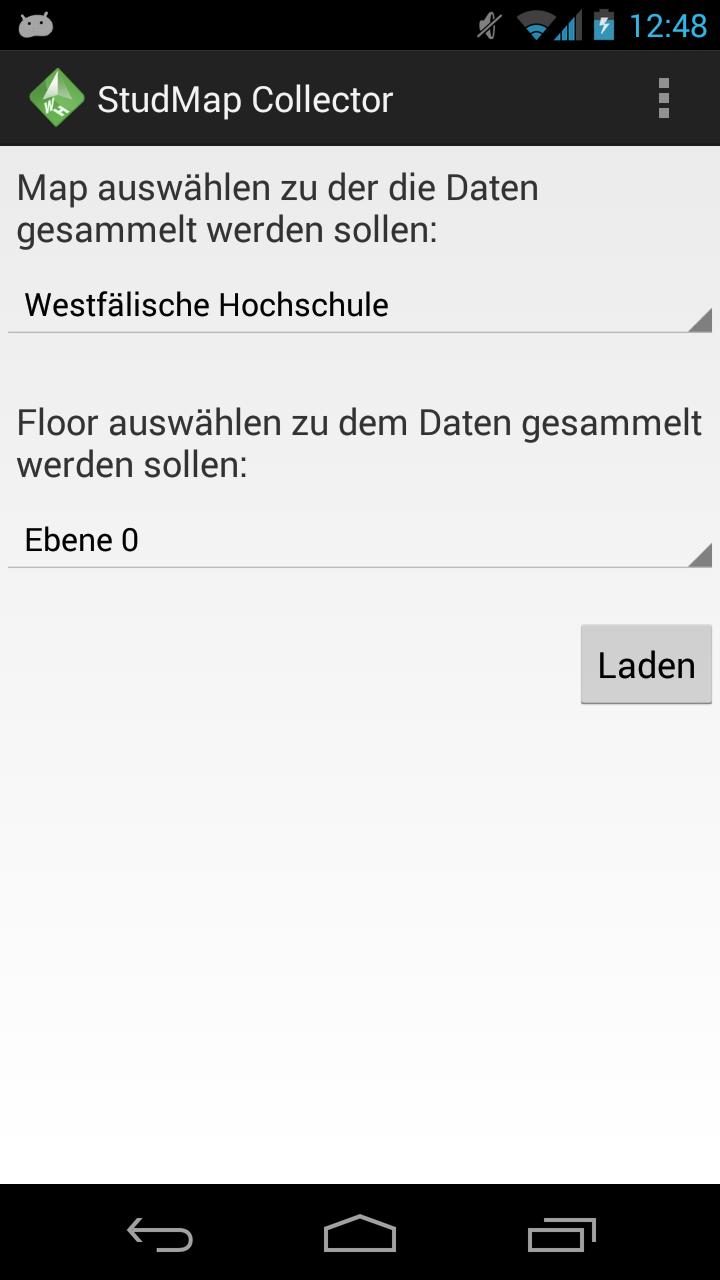
\includegraphics[width=0.5\linewidth]{../Bilder/Collector/StartScreen}
\label{fig:StartScreen}
\end{figure}
Hier k�nnen Karte und Stockwerk f�r die Datenerfassung ausgew�hlt werden. �ber den Button \textit{Laden} wird die entsprechende Auswahl geladen.

\newpage

\subsection{Stockwerkansicht}
Hier sieht man das ausgew�hlte Stockwerk mit den zur Verf�gung stehenden Punkten, die gr�n dargestellt sind.
\begin{figure}[H]
\centering
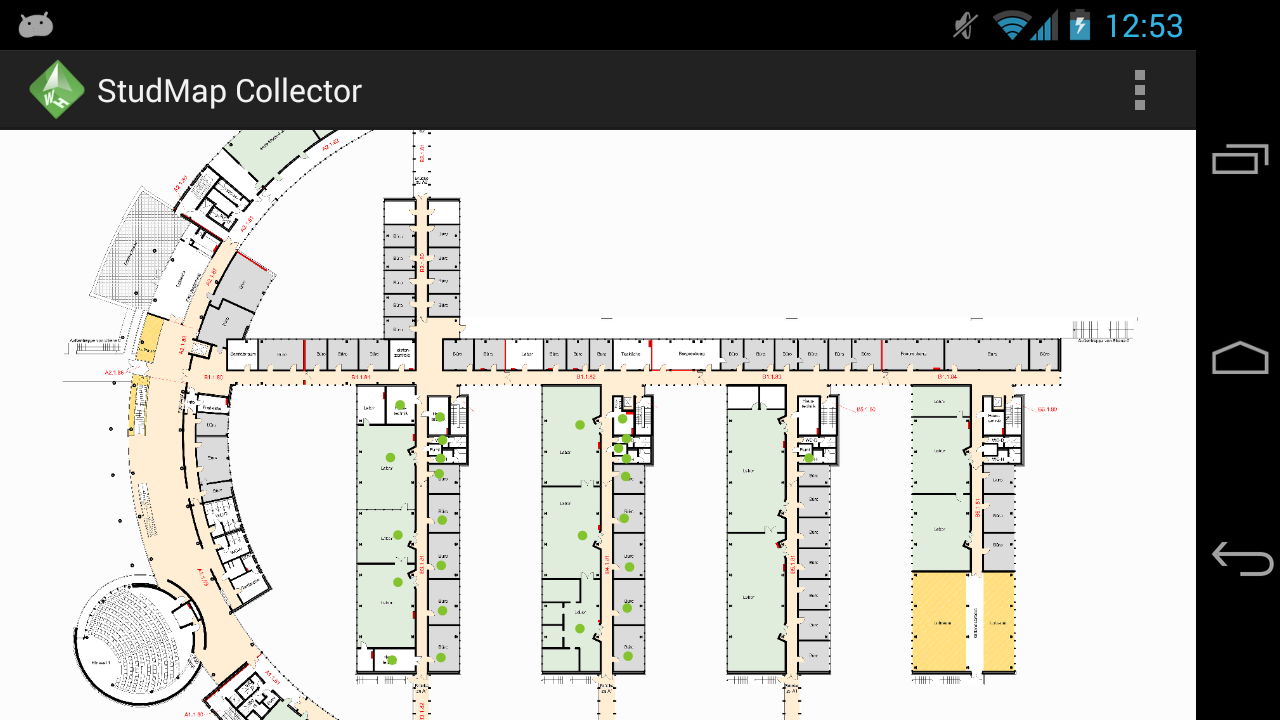
\includegraphics[width=0.8\linewidth]{../Bilder/Collector/FloorScreen}
\label{fig:FloorScreen}
\end{figure}

\subsubsection{Punktauswahl}
Bei der Auswahl eines Punktes erscheint folgender Dialog:
\begin{figure}[H]
\centering
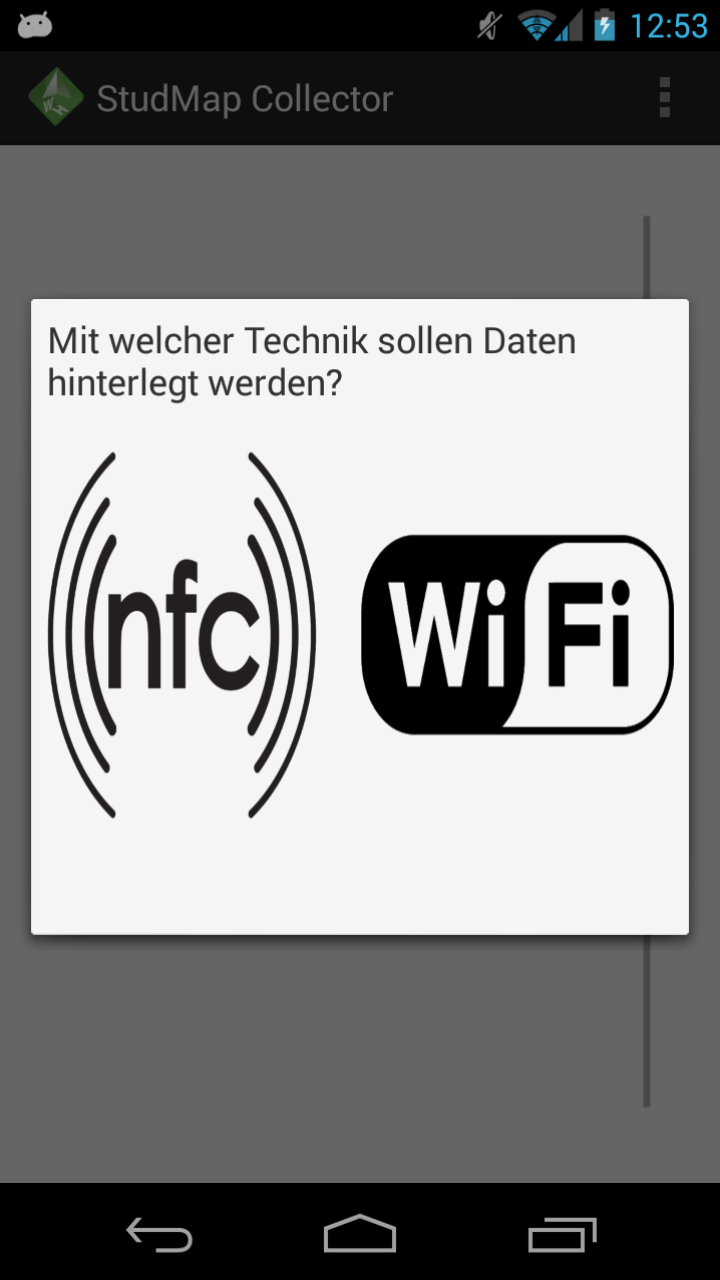
\includegraphics[width=0.35\linewidth]{../Bilder/Collector/StoreDataScreen}
\label{fig:StoreDataScreen}
\end{figure}
�ber diesen Dialog k�nnen f�r den ausgew�hlten Punkt Positionsdaten hinterlegt werden. Dazu stehen die beiden Techniken NFC und WiFi zur Verf�gung.

\paragraph{NFC-Tag Ansicht}
\textit{ }\\
Solange das Ger�t keinen Kontakt zu einem NFC-Tag hat, wird nur die ID des Punktes ausgegeben.
\begin{figure}[H]
\centering
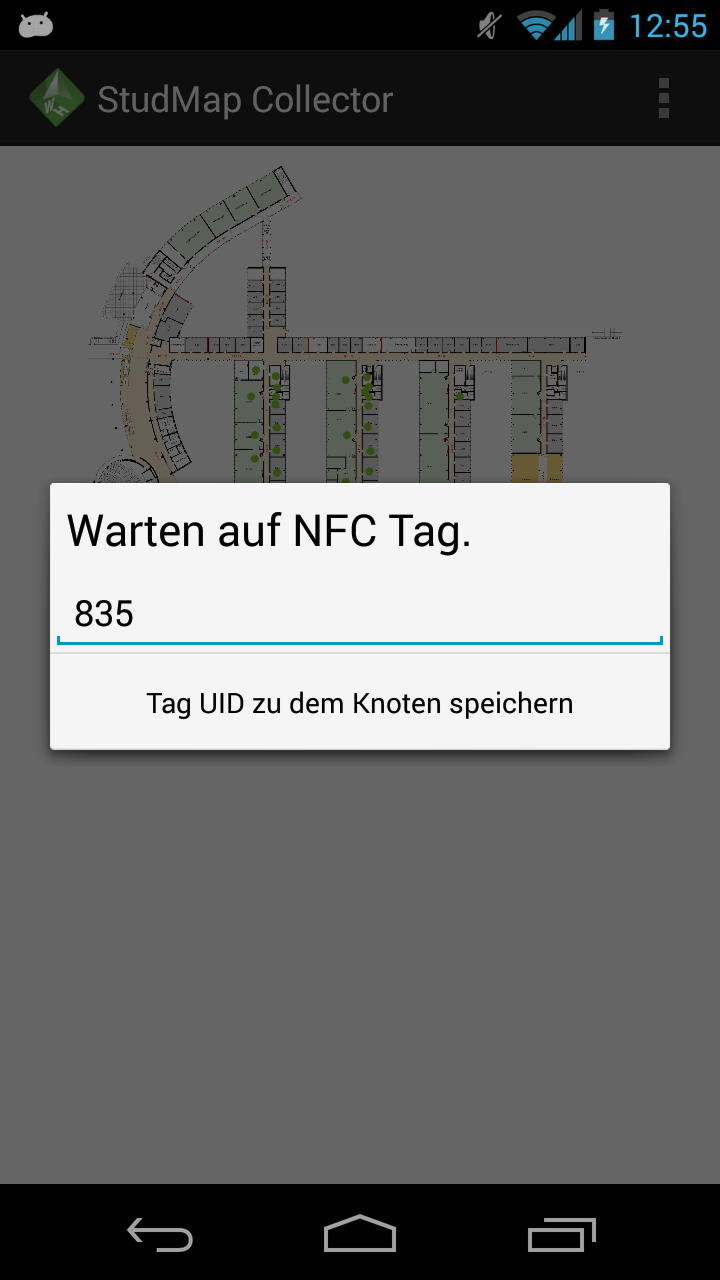
\includegraphics[width=0.35\linewidth]{../Bilder/Collector/NfcScreen}
\label{fig:NfcScreen}
\end{figure}

Sobald ein NFC-Tag gefunden wurde, wird auch die UID des NFC-Tags im Dialog angezeigt und der Datenpunkt kann mit dem NFC-Tag verkn�pft werden.
\begin{figure}[H]
\centering
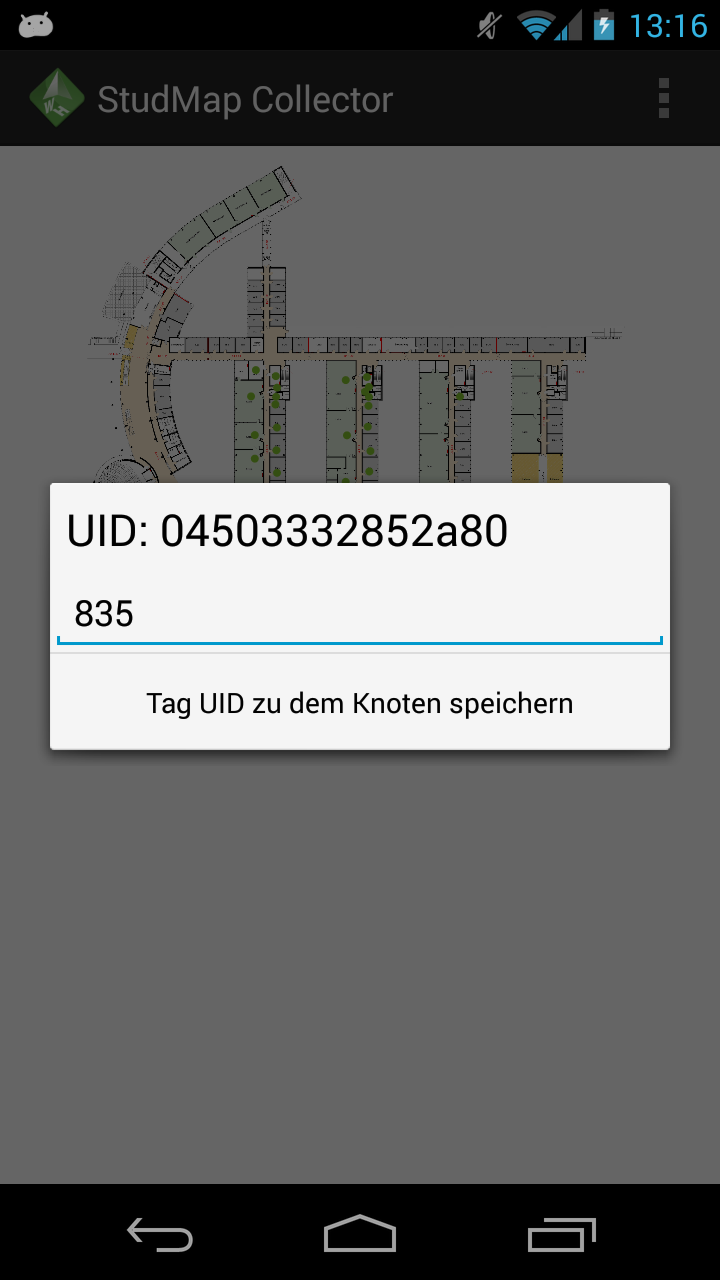
\includegraphics[width=0.35\linewidth]{../Bilder/Collector/NfcScreenRead}
\label{fig:NfcScreenRead}
\end{figure}

\newpage

\paragraph{WiFi}
\textit{ }\\
�ber diesen Dialog kann f�r den ausgew�hlten Punkt ein WLAN-Fingerprint erstellt und gespeichert werden.
\begin{figure}[H]
\centering
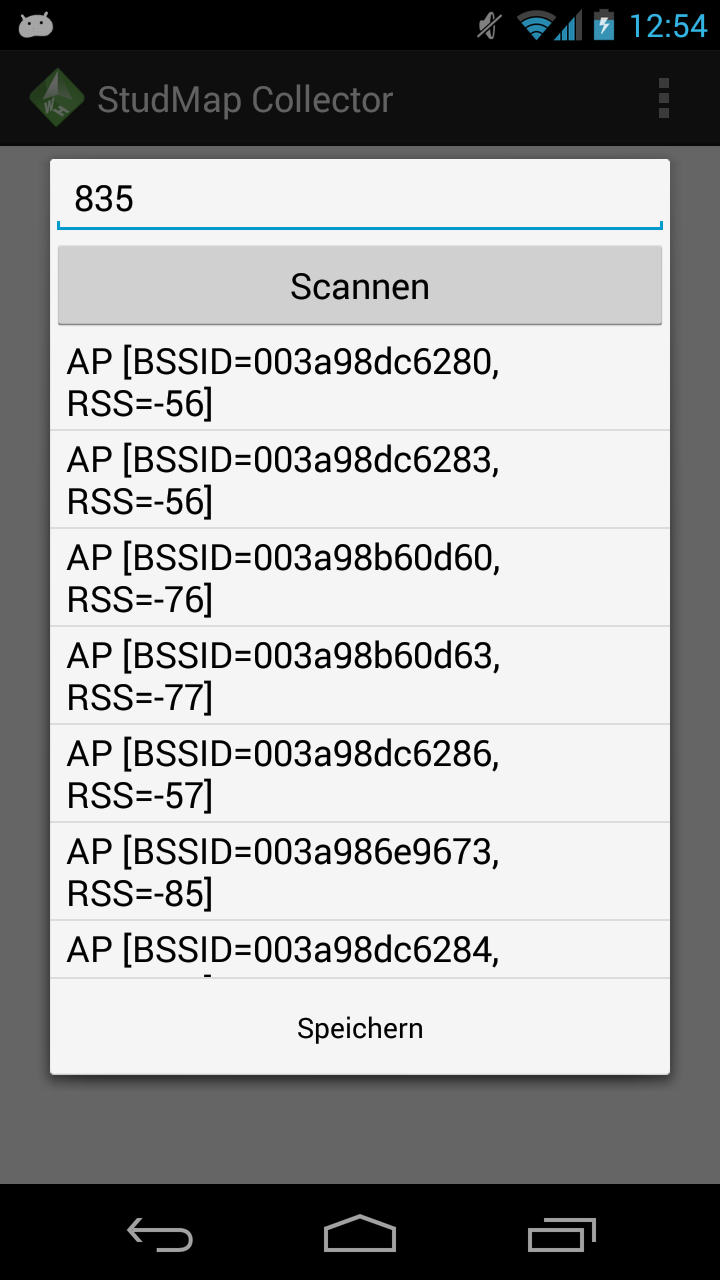
\includegraphics[width=0.5\linewidth]{../Bilder/Collector/WifiScannedScreen}
\label{fig:WifiScannedScreen}
\end{figure}
